% Compilar desde esta carpeta: pdflatex memoria_teoria; bibtex memoria_teoria;
% pdflatex memoria_teoria; pdflatex memoria_teoria.
\documentclass[11pt,a4paper]{article}
\usepackage[utf8]{inputenc}
\usepackage[T1]{fontenc}
\usepackage[spanish,es-nodecimaldot]{babel}
\usepackage{amsmath,amssymb,bm,booktabs,geometry,array,graphicx,longtable}
\geometry{margin=2.4cm}
\emergencystretch=2em
\newcommand{\ket}[1]{|#1\rangle}
\newcommand{\bra}[1]{\langle #1|}
\newcommand{\braket}[2]{\langle #1|#2\rangle}
\newcommand{\ee}{\mathrm{e}}
\newcommand{\ii}{\mathrm{i}}
\newcommand{\wb}{\omega_b}
\newcommand{\gphi}{\gamma_\varphi}
\newcommand{\Dxx}{\Delta_{xx}}
\DeclareMathOperator{\sinc}{sinc}

\title{Memoria de fonones en una molécula excitónica de tres puntos:\\ modelo, derivaciones, resultados y límites}
\author{}
\date{Documento de trabajo --- 17 de octubre de 2026}

\begin{document}
\maketitle

\noindent\textbf{Alcance.} Este documento reúne el modelo, las derivaciones, los resultados numéricos y sus
limitaciones para una memoria fonónica de tres emisores acoplados por Förster. El protocolo principal guarda
un qubit de dos \emph{time-bins} en dos estados oscuros y utiliza un modo acústico. La variante A1 de dos
modos y codificación en frecuencia se trata por separado. Las fuentes de datos son
\texttt{RESULTADOS\_F7\_F9\_MEMORIA\_RAMAN.md},
\texttt{RESULTADOS\_F14\_COVARIANZA\_ESPACIAL.md},
\texttt{RESULTADOS\_F18\_LAMBDA.md}, \texttt{RESULTADOS\_A1\_CONTROLES.md} y \texttt{RESULTADOS\_FEM\_AXISIMETRICO.md}.
Unidades: $\hbar=1$, $\wb=1$; a $f_b=100$~GHz, $1/\wb=1.59$~ps y $2000/\wb\simeq 3.2$~ns.
Las estimaciones geométricas son cotas o modelos simplificados, no una demostración de que un dispositivo
reúna todos los parámetros.

%==========================================================================
\section{Modelo}
Tres puntos cuánticos $i=1,2,3$ (dos niveles, operadores $\sigma_i$, $n_i=\sigma_i^\dagger\sigma_i$) y un modo
acústico $b$:
\begin{align}
H &= \wb\, b^\dagger b + \sum_{ij} h_{ij}\,\sigma_i^\dagger\sigma_j + \Dxx\sum_{i<j} n_in_j
 + \sum_i \lambda_i n_i (b+b^\dagger) + H_L(t), \label{eq:H}\\
H_L &= \frac{\Omega(t)}{\sqrt3}\sum_i\big(\sigma_i\,\ee^{\ii\omega_L t}+\mathrm{h.c.}\big),
\end{align}
con $h_{ii}=\varepsilon_i$ (energías de sitio, ajustables por efecto Stark) y $h_{i\neq j}=J_{ij}$ (Förster).
El término $\Dxx$ es la energía de interacción por par de excitones (biexcitón).
En el marco que gira con el láser, $H\to H-\omega_L N$ con $N=\sum_i n_i$.
La disipación es de tipo Lindblad con $\dot\rho=-\ii[H,\rho]+\sum_k D[L_k]\rho$, $D[L]\rho=L\rho L^\dagger-\tfrac12\{L^\dagger L,\rho\}$:
\begin{equation}
L_\kappa=\sqrt{\kappa}\,b,\quad
L_\gamma=\sqrt{2\gamma/3}\textstyle\sum_i\sigma_i,\quad
L_\varphi^{(\alpha)}=\sqrt{\gphi\,\mu_\alpha}\textstyle\sum_i u_{i\alpha}n_i,\quad
L_{b\leftarrow a}=\sqrt{\Gamma_{a\to b}}\textstyle\sum_{ij}b_ia_j\,\sigma_i^\dagger\sigma_j .
\label{eq:lind}
\end{equation}
Aquí $L_\gamma$ representa emisión radiativa colectiva de dipolos paralelos y en fase,
$(\mu_\alpha,u_\alpha)$ son autovalor y autovector de la matriz de correlación del desfase $K$ (sección~\ref{sec:ruido}),
y $L_{b\leftarrow a}$ describe la relajación por el continuo de fonones entre estados de un excitón (sección~\ref{sec:continuo}).
La normalización escogida da una tasa de población radiativa $2\gamma$ para $\ket B$ y cero para un oscuro ideal.
En el modelo reducido se proyecta el espacio electrónico a $\{G,B,D_1,D_2\}$, se excluyen dos y tres
excitones y se usan saltos $\sqrt{\Gamma_{a\to b}}\ket b\!\bra a$; en el modelo completo se conservan
los ocho estados electrónicos y el término biexcitónico. Esas dos implementaciones no son idénticas
fuera del sector de un excitón, como muestran los controles F16b--F17b.

\paragraph{Temperatura.} Las corridas principales son a $T_{\rm bath}=0$. Para un baño térmico del modo
deben añadirse $L_-=\sqrt{\kappa(n_{\rm th}+1)}b$ y
$L_+=\sqrt{\kappa n_{\rm th}}b^\dagger$, con
$n_{\rm th}=[\exp(\hbar\wb/k_BT_{\rm bath})-1]^{-1}$, y los factores de emisión/absorción
correspondientes en $\Gamma_{a\to b}$. A $100$~GHz, $\hbar\wb/k_B\simeq4.80$~K:
$n_{\rm th}\simeq0.008$ a $1$~K y $\simeq1.1\times10^{-7}$ a $0.3$~K.
El documento no contiene una corrida térmica completa de esta memoria; no se extrapola el rendimiento
de $T_{\rm bath}=0$ a esas temperaturas.

%==========================================================================
\section{Base de un excitón: estado brillante y estados oscuros}\label{sec:base}
En el sector de un excitón $H$ se reduce a la matriz $3\times3$ $h=(h_{ij})$. El láser con amplitud idéntica y fase común
en cada punto solo crea el estado simétrico
\begin{equation}
\ket{B}=\tfrac1{\sqrt3}(1,1,1),\qquad \ket{G}\to\ket{B}:\ \ \langle B|\textstyle\sum_i\sigma_i^\dagger|G\rangle=\sqrt3 .
\end{equation}
\paragraph{Condición de oscuridad.}
Los dos estados ortogonales a $\ket B$ no se acoplan al láser ni a la emisión colectiva
($L_\gamma\ket{D}=0$, $H_L\ket{D}\propto\ket{G}\!\bra{D}$ nulo). Para que sean además \emph{autoestados} de $h$
(oscuridad exacta, sin mezcla coherente con $\ket B$) es necesario y suficiente que $\ket B$ sea autovector de $h$,
es decir, que todas las filas de $h$ sumen lo mismo: $\sum_j h_{ij}=E_B$ para todo $i$.

\paragraph{Construcción inversa.}
Se pide $\ket B$ con energía $E_B=0$ y dos estados oscuros ortonormales
\begin{equation}
\ket{D_1}=\tfrac1{\sqrt2}(0,1,-1),\qquad \ket{D_2}=\tfrac1{\sqrt6}(2,-1,-1),
\end{equation}
con energías $E_1=-G_1$, $E_2=-G_2$ ($0<G_1<G_2$; ambos por debajo del brillante, véase la sección~\ref{sec:raman}).
La letra $G_s$ designa la \emph{brecha excitónica}; $g_s$ designará exclusivamente el elemento de matriz fonón--brillante--oscuro.
Entonces $h=\sum_aE_a\ket a\!\bra a$ da, elemento a elemento,
\begin{align}
h_{11}&=\tfrac13(E_B+2E_2)=-\tfrac23 G_2, &
h_{22}=h_{33}&=\tfrac13E_B+\tfrac12E_1+\tfrac16E_2=-\tfrac12G_1-\tfrac16G_2,\nonumber\\
J_{12}=J_{13}&=\tfrac13(E_B-E_2)=\tfrac13 G_2, &
J_{23}&=\tfrac13E_B-\tfrac12E_1+\tfrac16E_2=\tfrac12G_1-\tfrac16G_2 . \label{eq:jeps}
\end{align}
Se comprueban las sumas por fila: $\varepsilon_1+2J_{12}=0$ y $\varepsilon_2+J_{12}+J_{23}=0$, y además
$\varepsilon_1-\varepsilon_2=J_{23}-J_{12}$.
Para el punto de trabajo $(G_1,G_2)=(0.35,0.6)\wb$: $\varepsilon_1=-0.400$, $\varepsilon_2=\varepsilon_3=-0.275$,
$J_{12}=J_{13}=0.200$, $J_{23}=0.075$ (en unidades de $\wb$).

\paragraph{Consecuencia geométrica.}
Si $J_{ij}\propto r_{ij}^{-3}$ con la misma orientación dipolar, el cociente de lados del triángulo isósceles es
\begin{equation}
\Big(\frac{r_{23}}{r_{12}}\Big)^{3}=\frac{J_{12}}{J_{23}}=\frac{2G_2}{3G_1-G_2},
\qquad \frac{r_{23}}{r_{12}}\Big|_{(0.35,0.6)}=1.39 .
\end{equation}
Solo $G_1=G_2$ corresponde al triángulo equilátero, pero entonces $\ket{D_1},\ket{D_2}$ son degenerados y la ranura no se
puede seleccionar por frecuencia. Los cálculos de relajación de F11--F13 usaron un triángulo equilátero; la corrección está
en la sección~\ref{sec:continuo}.

\paragraph{Escala de energías.}
A $f_b=100$~GHz, $\hbar\wb=0.4136$~meV; con $J_{12}=0.2\wb=0.083$~meV y la escala dipolar de $0.13$~meV a $6$~nm
(teórica, Sirkina et al.~\cite{sirkina2025}) se obtiene $r_{12}\simeq7.0$~nm y $r_{23}\simeq9.7$~nm.
Es una estimación de orden de magnitud que presupone orientación dipolar y ausencia de túnel.

%==========================================================================
\section{Acoplo fonón--excitón en la base propia}\label{sec:fonon}
Sea $\Lambda=\mathrm{diag}(\lambda_1,\lambda_2,\lambda_3)$ y $V=\Lambda_{\mathrm{ex}}(b+b^\dagger)$ con
$\Lambda_{\mathrm{ex}}=\sum_i\lambda_i n_i$. En el sector de un excitón, $\langle a|\Lambda|b\rangle=\sum_i\lambda_i a_ib_i$:
\begin{align}
g_1&\equiv\langle B|\Lambda|D_1\rangle=\frac{\lambda_2-\lambda_3}{\sqrt6},\qquad
g_2\equiv\langle B|\Lambda|D_2\rangle=\frac{2\lambda_1-\lambda_2-\lambda_3}{\sqrt{18}},\label{eq:g}\\
\langle D_1|\Lambda|D_2\rangle&=-\frac{\lambda_2-\lambda_3}{\sqrt{12}}=-\frac{g_1}{\sqrt2},\nonumber\\
\langle B|\Lambda|B\rangle&=\frac{\lambda_1+\lambda_2+\lambda_3}{3},\quad
\langle D_1|\Lambda|D_1\rangle=\frac{\lambda_2+\lambda_3}2,\quad
\langle D_2|\Lambda|D_2\rangle=\frac{4\lambda_1+\lambda_2+\lambda_3}{6}.\nonumber
\end{align}
Solo la parte \emph{no uniforme} de $\lambda_i$ acopla el brillante con los oscuros; la parte uniforme $\bar\lambda$
solo desplaza el modo (polarón). Es el mecanismo de transferencia transversal ($b\,\sigma_{DB}^\dagger+\mathrm{h.c.}$) que
un emisor único no tiene.
Con $\bm\lambda=(0.20,0.14,0)\wb$: $g_1=0.0572$, $g_2=0.0613$, $\langle D_1|\Lambda|D_2\rangle=-0.0404$.

\section{Qué se almacena y por qué se necesitan tres emisores}\label{sec:protocolo}
La entrada principal es un qubit de un fonón en dos tiempos, entrelazado con una referencia que no
interactúa con la memoria:
\begin{equation}
\ket{\Psi_{\rm in}}=\frac{\ket{0}_R\ket{1_{t_1},0_{t_2}}+\ket{1}_R\ket{0_{t_1},1_{t_2}}}{\sqrt2}.
\end{equation}
La primera ventana carga el modo y un pulso Raman escribe $\ket{G,1}\to\ket{D_1,0}$; la segunda
escribe la otra rama en $D_2$. Durante la espera el subespacio lógico es
$\mathcal H_L=\mathrm{span}\{\ket{D_1,0},\ket{D_2,0}\}$, con una excitación electrónica en ambas ramas.
La lectura invierte el orden de los pulsos y devuelve el fonón a dos ventanas de salida. El láser
está apagado en la espera; al estar $D_s$ por debajo de $B$ y lejos de la resonancia de un fonón,
la memoria Raman no requiere apagar el intercambio Förster. La transferencia es una transición
\emph{estimulada} entre un fonón y una excitación oscura; no es una cascada espontánea de Stokes
ni la emisión de paquetes de Bin et al.

Con dos emisores y excitones de dos niveles hay un brillante y un oscuro: puede almacenarse una
ocupación en $D$, pero una superposición $\ket G+\ket D$ compara sectores con $N=0$ y $N=1$,
por lo que el ruido común conserva su desfase $\gphi/2$. Tres emisores dan dos oscuros ortogonales
en el \emph{mismo} sector $N=1$; el ruido proporcional a $N$ desplaza ambos igual. Esta protección
no cubre los intervalos de carga y lectura secuenciales, cuando solo una rama ya contiene un excitón.
En un qubit de frecuencia con dos modos cargados simultáneamente (A1), ese intervalo se reduce,
pero A1 es un protocolo distinto y sus cifras no sustituyen las del qubit temporal.

El producto físico de escritura, espera y lectura se evalúa como un canal con pérdida. Si $\rho_{R,\rm out}$
es el estado de referencia y salida incluyendo el vacío, $s=\mathrm{Tr}(\Pi_{1}\rho_{R,\rm out})$
es la probabilidad de recuperar un fonón en las ventanas lógicas, $F=\bra{\Psi_{\rm id}}
\rho_{R,\rm out}\ket{\Psi_{\rm id}}$ es la fidelidad \emph{sin} condicionar, y
$F_h=F/s$ es la fidelidad condicionada a esa recuperación. Por ello $F=sF_h$; una ventaja en
$F$ puede proceder de mayor éxito aunque $F_h$ sea menor que la referencia pasiva.

%==========================================================================
\section{Transferencia Raman fonón $\leftrightarrow$ excitón oscuro}\label{sec:raman}
\subsection{Hamiltoniano efectivo}
Consideramos un fonón en el modo y el láser a frecuencia $\omega_L$. En el marco rotante, con $\delta_x=E_x-\omega_L$,
los estados relevantes son
\begin{equation}
\ket{G,1}\ (\text{energía }\wb),\qquad \ket{B,1}\ (\delta_B+\wb),\qquad \ket{D_s,0}\ (\delta_s),
\end{equation}
acoplados por $\langle B,1|H_L|G,1\rangle=\Omega$ y $\langle B,1|V|D_s,0\rangle=g_s$ (tomando solo la parte que
conserva la excitación, $|B\rangle\langle D_s|\,b^\dagger$).
La resonancia de dos fotones es $\delta_s=\wb+\delta_2$, con $\delta_2$ pequeña. El detuning del intermedio es
\begin{equation}
\Delta_I\equiv(\delta_B+\wb)-\wb=\delta_B=\delta_s-\mathrm{gap}_s=\wb+\delta_2+|{\rm gap}_s| ,
\qquad \mathrm{gap}_s=E_{D_s}-E_B<0,
\end{equation}
que \emph{siempre es grande} si el estado oscuro está por debajo del brillante ($\delta_B>\wb$).
Eliminando adiabáticamente $\ket{B,1}$ ($\Omega,g_s\ll\Delta_I$) se obtiene en $\{\ket{G,1},\ket{D_s,0}\}$
\begin{equation}
H_{\rm eff}=\begin{pmatrix}\wb-\Omega^2/\Delta_I & -\Omega_{\rm eff}\\[2pt] -\Omega_{\rm eff} & \wb+\delta_2-g_s^2/\Delta_I\end{pmatrix},
\qquad \Omega_{\rm eff}=\frac{\Omega\,g_s}{\Delta_I}.
\label{eq:Heff}
\end{equation}
\paragraph{Resonancia corregida por desplazamiento de luz.}
La resonancia efectiva es $\delta_2^\star=(g_s^2-\Omega^2)/\Delta_I$ y la transferencia completa de $\ket{G,1}$ a $\ket{D_s,0}$
ocurre en el tiempo $\pi$
\begin{equation}
t_\pi=\frac{\pi}{2\Omega_{\rm eff}}=\frac{\pi\Delta_I}{2\Omega g_s}. \label{eq:tpi}
\end{equation}
La población del intermedio es $p_B\simeq(\Omega/\Delta_I)^2\cos^2$-modulada; la pérdida radiativa de la transferencia es
$\simeq 2\gamma\,p_B\,t_\pi\sim10^{-3}$ y se desprecia.

\paragraph{Pérdida del fonón durante la escritura.}
Mientras dura la transferencia el fonón sigue en el modo con $P_{G1}(t)=\cos^2(\Omega_{\rm eff}t)$ y se pierde a tasa $\kappa$:
\begin{equation}
1-\eta_w\simeq\kappa\!\int_0^{t_\pi}\!\cos^2(\Omega_{\rm eff}t)\,\mathrm{d}t=\frac{\kappa t_\pi}{2}
\quad\Rightarrow\quad \eta_w\simeq1-\frac{\pi\kappa\Delta_I}{4\Omega g_s}. \label{eq:etaw}
\end{equation}
Esto impone un compromiso: reducir $\Delta_I$ acorta $t_\pi$ pero aumenta la población virtual del brillante, que se desfasa y relaja ($p_B\sim(\Omega/\Delta_I)^2$).

\paragraph{Separación modal óptima con dos modos (codificación en frecuencia).}
Si el qubit se codifica en dos modos $\omega_1,\omega_2$ y las dos rutas Raman $|G,1_s\rangle\to|D_s,0\rangle$ comparten un láser, el intermedio queda a $\Delta_I=-\omega_L$ en las dos y
\begin{equation}
\omega_1-\omega_2=(E_{D_1}-E_{D_2})-(\delta^\star_{2,1}-\delta^\star_{2,2}),\qquad
\delta^\star_{2,s}=-\frac{\Omega^2}{\Delta_I}+\sum_{m=1,2}\sum_{c}\frac{|\Lambda^{(m)}_{cs}|^2}{\omega_m+E_c-E_s},
\end{equation}
autoconsistente en $\omega_{1,2}$. Para $\bm\lambda=(0.20,0.14,0)$ da $0.288$ ($\Omega=0.20$, $\omega_L=-1.485$) y $0.259$ ($\Omega=0.39$, $\omega_L=-1.380$), frente a $0.290$ y $0.260$ de la optimización numérica (y $0.250$ sin corrección).
La tolerancia a un error en la separación es de $\sim\pm0.01\,\wb$ (pérdida de $F$ de $0.06$--$0.08$ en la escritura cerrada).

\paragraph{Escala del acoplo mínimo.}
Como $\Omega_{\rm eff}=\Omega g/\Delta_I$ y $p_B=(\Omega/\Delta_I)^2$ es la población virtual del brillante, a tiempo $t_\pi$ fijo ($\Omega_{\rm eff}=\pi/2t_\pi$) el acoplo necesario es
\begin{equation}
g_{\min}=\frac{\Omega_{\rm eff}}{\sqrt{p_{B,\max}}}=\frac{\pi}{2\,t_\pi\sqrt{p_{B,\max}}},\qquad \Omega=\Omega_{\rm eff}\Delta_I/g\ \propto\ 1/g,
\label{eq:gmin}
\end{equation}
de modo que reducir $\lambda$ obliga a subir $\Omega\propto1/\lambda$ con la duración casi fija. Para $t_\pi\simeq190/\wb$: $g_{\min}=0.026$ ($p_{B,\max}=0.1$) o $0.019$ ($0.2$).
Un barrido de $\lambda$ con pulsos reoptimizados (F18) lo confirma: $S=0.5$ ($g\simeq0.03$, $p_B=0.09$) conserva $F_h=0.84$ con entrada/salida reales, $S=0.33$ ($g\simeq0.02$, $p_B=0.2$) baja a $0.73$.

\paragraph{Fuga hacia la otra ranura.}
Con el láser sintonizado a la ranura $s$, la otra ranura $s'$ queda desintonizada en dos fotones por $\Delta_{ss'}=|E_{D_s}-E_{D_{s'}}|$ con acoplo efectivo $\Omega_{\rm eff}'=\Omega g_{s'}/\Delta_I$.
La población máxima que alcanza es la de un oscilador de Rabi desintonizado,
\begin{equation}
P_{s'}^{\max}=\frac{(2\Omega_{\rm eff}')^2}{(2\Omega_{\rm eff}')^2+\Delta_{ss'}^2}\simeq\frac{4\Omega_{\rm eff}'^2}{\Delta_{ss'}^2}\approx5\times10^{-3}
\end{equation}
para $\Omega_{\rm eff}'=0.0091$ y $\Delta_{ss'}=0.25$; coincide con la diafonía de $\sim0.005$--$0.01$ de la figura de dinámica Raman
(una estimación previa con $(\Omega'_{\rm eff}/\Delta_{ss'})^2\sim10^{-3}$ omitía el factor 4).

\paragraph{Rizado por admixtura del brillante.}
Durante el pulso, $\ket{G,1}$ y $\ket{D_s,0}$ se mezclan con $\ket{B,1}$ con amplitud $\Omega/\Delta_I$, y esa mezcla oscila a la frecuencia $\Delta_I$ (periodo $2\pi/\Delta_I\simeq4.7/\wb$).
De ahí el rizado de amplitud $\sim(\Omega/\Delta_I)^2\simeq2$\,\% en la población de $\ket{D_s,0}$ frente a la duración del pulso, y el que la fidelidad dependa de la fase del apagado.
Un apagado \emph{adiabático} (rampa de duración $\gg\Delta_I^{-1}$) suprime el rizado y recuperaría ese $\sim2$\,\% de $\eta_w$.

\paragraph{Corrección polarónica de la resonancia.}
El estado $\ket{G,1}$ no se acopla al fonón (no hay excitón), pero $\ket{D_s,0}$ sí lo hace con \emph{todos} los estados $\ket{c,1}$ del sector de un excitón
($c=B,D_1,D_2$, incluido $c=s$ por el elemento diagonal $\langle D_s|\Lambda|D_s\rangle$). Al segundo orden en $\Lambda$ la energía de $\ket{D_s,0}$ se desplaza en
$-\sum_c|\Lambda_{cs}|^2/(\wb+E_c-E_s)$ y la condición $E'_{G1}=E'_{D_s0}$ da
\begin{equation}
\delta_2^\star=-\frac{\Omega^2}{\Delta_I}+\sum_{c\in\{B,D_1,D_2\}}\frac{|\Lambda_{cs}|^2}{\wb+E_c-E_s}. \label{eq:d2star}
\end{equation}
El término $c=B$ es el de la Ec.~\eqref{eq:Heff}; el diagonal ($c=s$) es el desplazamiento de polarón $\ell_s^2/\wb$ y es el que domina para $s=D_2$ porque $\langle D_2|\Lambda|D_2\rangle=0.157$.

\subsection{Comparación con la simulación (F13, arranque 1; $\kappa=10^{-3}$)}
\begin{center}\small
\begin{tabular}{lccccccc}\toprule
ranura & $\Omega$ & $g_s$ & $\Delta_I$ & $t_\pi$ teoría & $t_\pi$ sim. & $\delta_2^\star$ primer orden & $\delta_2^\star$ Ec.~\eqref{eq:d2star} / sim.\\\midrule
1 ($G_1{=}0.35$) & 0.197 & 0.0572 & 1.33 & 185 & 170 & $-0.0267$ & $-0.0197$ / $-0.020$\\
2 ($G_2{=}0.60$) & 0.290 & 0.0613 & 1.575 & 139 & 150 & $-0.0510$ & $-0.0252$ / $-0.025$\\\bottomrule
\end{tabular}
\end{center}
El tiempo $\pi$ se reproduce a $\lesssim10$\,\%. La resonancia con la corrección de polarón coincide con la simulación a $\lesssim5\times10^{-4}\,\wb$ en ambas ranuras;
el desajuste de un factor~2 de la estimación de primer orden en la ranura~2 se debía al término diagonal $\ell_2^2/\wb=0.0245$.

\paragraph{Presupuesto de la escritura.}
La simulación da $0.841$ de población en $D_1$ tras escribir; dividiendo por la eficiencia de carga $\eta_L=0.9613$ (la rama $R=0$ incluye el $3.9$\,\% no cargado) resulta $\eta_w=0.875$.
El modelo analítico con pulso finito y pérdida $\kappa$:
\begin{equation}
\eta_w\simeq\sin^2(\Omega_{\rm eff}d)\,\Big[1-\kappa\Big(\frac d2+\frac{\sin 2\Omega_{\rm eff}d}{4\Omega_{\rm eff}}\Big)\Big]=0.983\times0.907=0.892,
\end{equation}
con $d=170$, $\Omega_{\rm eff}=0.00847$. El residuo ($1.7$\,\%) es del orden de la admixtura del brillante, $(\Omega/\Delta_I)^2=2.2$\,\%, que se pierde al apagar el pulso de forma abrupta.

%==========================================================================
\section{Ruido de desfase: correlación espacial y coherencia del doble carril}\label{sec:ruido}
\subsection{Modelo de ruido}
Se supone ruido gaussiano blanco $\xi_i(t)$ que desplaza la energía del punto $i$ con
$\langle\xi_i(t)\xi_j(t')\rangle=\gphi K_{ij}\,\delta(t-t')$, $K$ semidefinida positiva con $K_{ii}=1$. Diagonalizando
$K=\sum_\alpha\mu_\alpha u_\alpha u_\alpha^{\!T}$ se obtienen los saltos $L_\varphi^{(\alpha)}$ de la Ec.~\eqref{eq:lind}.
Casos: $K=\mathbb 1$ (local), $K=\bm1\bm1^{T}$ (común), $K=(1-\chi)\mathbb 1+\chi\bm1\bm1^{T}$ (mezcla), $K=\bm\alpha\bm\alpha^{T}$ (común con respuestas Stark $\alpha_i$).

\subsection{Resultado exacto sin hopping}
Como los $n_i$ son diagonales en la base de sitios, el desfase solo multiplica por una fase aleatoria cada elemento:
\begin{equation}
\dot\rho_{ij}\big|_\varphi=-\Gamma_{ij}\rho_{ij},\quad \Gamma_{ij}=\tfrac12\gphi\,(K_{ii}+K_{jj}-2K_{ij}),\qquad
\dot\rho_{G\,i}\big|_\varphi=-\tfrac12\gphi K_{ii}\rho_{G\,i}.
\end{equation}
Para $K=(1-\chi)\mathbb1+\chi\bm1\bm1^T$: $\Gamma_{i\neq j}=\gphi(1-\chi)$ y la coherencia con el vacío decae a $\gphi/2$ \emph{para todo} $\chi$.
Una superposición de $\ket G$ con cualquier estado de un excitón (almacenamiento de un qubit vacío/un-fonón) no se protege con ruido común.

\subsection{Aproximación secular en la base propia}
Con $|E_a-E_b|\gg\gphi$, para un salto hermítico $A=\sum_i c_in_i$ (tasa $\gphi$) y $K=\bm c\bm c^T$, las poblaciones y coherencias de $\{B,D_1,D_2\}$ obedecen
\begin{align}
W_{a\leftrightarrow b}&=\gphi\sum_{ij}K_{ij}\,(n_i)_{ab}(n_j)_{ba},\qquad (n_i)_{ab}=a_ib_i,\label{eq:W}\\
\Gamma_{ab}&=\tfrac12\gphi\,w^{T}_{ab}Kw_{ab}+\tfrac12\Big(\sum_{c\ne a}W_{ac}+\sum_{c\ne b}W_{bc}\Big),\quad
(w_{ab})_i=|a_i|^2-|b_i|^2 .\label{eq:Gab}
\end{align}
El primer término es desfase puro; el segundo, la tasa a la que la amplitud sale por transiciones inducidas (el ruido blanco tiene espectro plano
y las induce aunque haya brecha; es una limitación del modelo markoviano, no física del ruido de carga de baja frecuencia).

\paragraph{Estados de la memoria de doble carril ($a=D_1,b=D_2$).}
Con los vectores de la sección~\ref{sec:base}: $w=\tfrac13(-2,1,1)$, $|w|^2=\tfrac23$, $\sum_iw_i=0$, y
$\sum_i(D_1^iD_2^i)^2=\tfrac16$, $\sum_i(B_iD_1^i)^2=\sum_i(B_iD_2^i)^2=\tfrac13$. Para $K=(1-\chi)\mathbb1+\chi\bm1\bm1^T$:
\begin{equation}
W_{D_1D_2}=\tfrac16\gphi(1-\chi),\quad W_{BD_{1,2}}=\tfrac13\gphi(1-\chi),\quad
\boxed{\Gamma_{D_1D_2}=\Big(\tfrac13+\tfrac12\Big)\gphi(1-\chi)=\tfrac56\,\gphi(1-\chi)} \label{eq:Gc}
\end{equation}
que se anula para $\chi=1$: el ruido común es una $N$ (operador $\sum n_i$ diagonal en la base propia) y no distingue las ranuras.

\paragraph{Respuestas Stark desiguales.}
Para $K=\bm\alpha\bm\alpha^T$ y $\alpha=(1+a,1,1)$: $w\!\cdot\!\alpha=-2a/3$, $\langle B|A|D_2\rangle=2a/\sqrt{18}$,
$\langle D_1|A|D_2\rangle=0$, y
\begin{equation}
\Gamma_{D_1D_2}(\alpha)=\tfrac12\gphi\tfrac{4a^2}{9}+\tfrac12\gphi\tfrac{4a^2}{18}=\tfrac13\gphi a^2 .
\end{equation}
Para $a=0.2$ y $T=8000$: $\Gamma T=0.043$, $\Delta F_h\simeq\tfrac12\mathcal V_0\Gamma T\approx0.019$ frente a $0.015$ de la simulación (F14b, $\alpha_1=1.2$);
para $a=0.1$: $0.005$ frente a $0.004$. La sensibilidad al desbalance es cuadrática.

\subsection{Ley de coherencia del doble carril}
Sea $P_r$ la probabilidad de éxito de la rama $r=0,1$ (fonón en el bin $r{+}1$). Con
$a=\tfrac12P_0$, $b=\tfrac12P_1$, $|c|=\tfrac12\sqrt{P_0P_1}\,\mathcal V$:
\begin{equation}
F=\tfrac12(a+b)+|c|=\tfrac14(P_0+P_1)+\tfrac12\sqrt{P_0P_1}\,\mathcal V,\qquad
s=\tfrac12(P_0+P_1),\qquad F_h=\frac Fs\ \xrightarrow{P_0=P_1}\ \tfrac12(1+\mathcal V).\label{eq:F}
\end{equation}
La visibilidad $\mathcal V$ acumula tres intervalos: (i) \emph{no protegidos} de escritura (ramas con $N=1$ y $N=0$), que decaen a $\gphi/2$;
(ii) de almacenamiento (ambas con $N=1$), tasa $\Gamma_{D_1D_2}$ (Ec.~\ref{eq:Gc}); (iii) \emph{no protegidos} de lectura:
\begin{equation}
\mathcal V=\mathcal V_0\exp\!\Big[-\tfrac12\gphi\,(\tau_{u}^{w}+\tau_{u}^{r})-\Gamma_{D_1D_2}\,T_{\rm prot}\Big],\qquad
\tau_u^{w}\simeq t_{L2}+\tau_{12}+\tfrac12 d_2,\ \ \tau_u^{r}\simeq t_E+tw .\label{eq:V}
\end{equation}
$\mathcal V_0$ recoge las imperfecciones de los pulsos independientes de los tiempos de espera.

\paragraph{Verificación (carga ideal, $\chi=1$, $T=2000$).}
\begin{center}\small
\begin{tabular}{rcccc}\toprule
$\tau_{12}$ & $F_h$ (simulación) & $\mathcal V=2F_h-1$ & $\mathcal V/\mathcal V(\tau_{12}{=}100)$ & $\exp[-\gphi(\tau_{12}-100)/2]$\\\midrule
100  & 0.932 & 0.864 & 1     & 1\\
400  & 0.898 & 0.796 & 0.921 & 0.942\\
1000 & 0.858 & 0.716 & 0.829 & 0.835\\
2000 & 0.788 & 0.576 & 0.667 & 0.684\\
4000 & 0.692 & 0.384 & 0.444 & 0.458\\\bottomrule
\end{tabular}
\end{center}
La pendiente de $\ln\mathcal V$ frente a $\tau_{12}$ coincide con $-\gphi/2=-2\times10^{-4}$ ($\gphi=4\times10^{-4}$); el exponente de la Ec.~\eqref{eq:V} queda verificado.
Con la lectura retardada ($tw=800$, F17b): $\mathcal V/\mathcal V_0=0.838$ frente a $\exp(-\gphi\,tw/2)=0.852$.


\subsection{Origen físico de la correlación $K_{ij}$: radio libre de trampas}\label{sec:trampas}
Sea ruido de carga producido por cargas puntuales (trampas) que desplazan la energía del punto $i$ por efecto Stark, $\delta E_i=\mu\,F_z(\bm r_i)$,
con $\bm r_i$ las posiciones de los puntos y $F_z$ la componente del campo a lo largo del eje de polarización, y $\mu$ el momento dipolar permanente (igual en todos).
Para una trampa en $\bm R$ (relativo al punto): $F_z\propto G(\bm R)=\cos\theta/R^2$. Si las trampas están distribuidas con densidad uniforme \emph{fuera} de una esfera de radio $r_0$ alrededor de la molécula,
\begin{equation}
K_{ij}=\frac{\int_{R>r_0}G(\bm R)\,G(\bm R-\bm d_{ij})\,\mathrm d^3R}{\int_{R>r_0}G^2\,\mathrm d^3R}\simeq1-c\,\frac{d_{ij}^2}{r_0^2},\qquad
c=\begin{cases}2/5 & \bm d_{ij}\parallel\hat z\\ 3/10 & \bm d_{ij}\perp\hat z\end{cases}\quad(d_{ij}\ll r_0).
\end{equation}
En efecto, $\int G^2=\tfrac{4\pi}{3r_0}$ y $\int(\partial_zG)^2=\tfrac{16\pi}{15r_0^3}$ (por $\int(1-3\cos^2\theta)^2\mathrm d\Omega=16\pi/5$), de donde $1-K=\tfrac12\,d^2\!\int(\partial G)^2/\!\int G^2=\tfrac25\,d^2/r_0^2$;
para separación perpendicular al eje se sustituye $16\pi/5\to12\pi/5$. Una integral de Monte Carlo confirma el coeficiente axial:
$1-K=0.0246,\ 0.00625,\ 0.00159$ para $r_0/d=4,8,16$ frente a $0.0250,\ 0.00625,\ 0.00156$.
Si las trampas llegan hasta el punto ($r_0\to0$), $K\to0$: la correlación espacial exige un volumen libre de carga de radio $r_0\gg d$.
El coeficiente $c$ depende de la orientación de cada par respecto al campo;
asignar un solo $c=0.3$--$0.4$ a todo el triángulo es una acotación,
no la covarianza de una geometría concreta ya resuelta. Una pila lineal
de tres puntos y un triángulo isósceles tienen distancias y matriz de
Förster diferentes; los valores de F14 no validan por sí solos el
diseño espectral de la Ec.~\eqref{eq:jeps}.

\paragraph{Consecuencia para el triángulo.}
Como $\sum_iw_i=0$ y $\sum_im_i=0$ para las formas que aparecen, solo importa la parte dependiente de $d_{ij}$ de $K$:
\begin{align}
w^TKw&=\frac{2c\,(4r^2-r'^2)}{9\,r_0^2},\qquad
\Gamma_{D_1D_2}=\gphi\,\frac{c\,(4r^2+r'^2)}{6\,r_0^2}\quad\text{(ruido blanco)}.
\end{align}
La segunda expresión suma el desfase puro $\tfrac12\gphi w^TKw$ y la mitad de las tasas de salida $W_{D_1D_2}=\gphi c\,r'^2/(6r_0^2)$, $W_{BD_1}=\gphi c\,r'^2/(3r_0^2)$, $W_{BD_2}=\gphi c\,(4r^2-r'^2)/(9r_0^2)$
(todas calculadas con $K_{ij}=1-cd_{ij}^2/r_0^2$ en la Ec.~\eqref{eq:W}). Con $r=6.98$, $r'=9.67$~nm ($c=0.3$--$0.4$) y $\gphi=4\times10^{-4}$:
$\Gamma_{D_1D_2}\,T\lesssim0.1$ a $T=2000$ pide $r_0\gtrsim12$~nm, y a $T=8000$ pide $r_0\gtrsim24$~nm.

\paragraph{Ruido cuasi-estático (baja frecuencia).}
Si el ruido es lento frente a $T$, el desplazamiento diferencial es una variable gaussiana por disparo con desviación $\sigma_\delta=\sigma_1\sqrt{w^TKw}$, donde $\sigma_1$ es la desviación Stark de un punto, y la visibilidad es
$\mathcal V=\mathcal V_0\,\ee^{-\sigma_\delta^2T_{\rm prot}^2/2}$. Con $\sigma_1=1~\mu$eV ($=2.4\times10^{-3}\wb$ a $100$~GHz) y $T_{\rm prot}=2300$: $\sigma_\delta T\lesssim0.5$ exige $w^TKw\lesssim8\times10^{-3}$, es decir
$r_0\gtrsim29$--$34$~nm (de $w^TKw=6.8$--$9.0\ \mathrm{nm}^2/r_0^2$ para $c=0.3$--$0.4$).

\paragraph{Intervalos no protegidos y escala de coherencia exigida.}
La coherencia entre $N=1$ y $N=0$ no la protege el ruido común (Sec.~\ref{sec:ruido}). Para ruido blanco requiere $\tfrac12\gphi\,\tau_u\lesssim0.1$, esto es $\gphi\lesssim0.2/\tau_u$ ($\gphi\lesssim3\times10^{-4}$ con $\tau_u=650$);
para ruido cuasi-estático requiere $\sigma_1\tau_u\lesssim0.5$ ($\sigma_1\lesssim0.3~\mu$eV con $\tau_u=650/\wb$ a 100~GHz).
Los anchos de línea típicos de puntos InAs/GaAs ($\sim1$--$5~\mu$eV, tomados de Borri et al.) son más grandes: o el intervalo no protegido debe acortarse hacia $\tau_u\sim200$--$300/\wb$ (puerto de carga $\kappa_{\rm in}\gtrsim30\kappa$ y $\tau_{12}$ mínimo; el piso lo fija $d_2/2\simeq75/\wb$ del pulso Raman), o hay que reducir el ruido de carga del dispositivo.
Este requisito, y no la correlación espacial, es la condición más exigente del esquema.

%==========================================================================
\section{Relajación por el continuo de fonones: regla de oro}\label{sec:continuo}
Acoplo deformación-potencial a fonones LA de volumen:
$H_{\rm ph}=\sum_{\bm q}M_q\,(c_{\bm q}+c_{-\bm q}^\dagger)\sum_i\ee^{\ii\bm q\cdot\bm r_i}n_i$, con densidad espectral
\begin{equation}
J(\omega)=\sum_{\bm q}|M_q|^2\delta(\omega-cq)=\frac{F(q)^2\,\omega^3}{4\pi^2\hbar\rho c^5},\quad
F(q)=D_e\ee^{-q^2a_e^2/4}-D_h\ee^{-q^2a_h^2/4},\ \ q=\omega/c .
\end{equation}
La tasa a $T=0$ de la transición $a\to b$ (energías $\omega_{ab}>0$, promedio isótropo sobre la dirección de $\bm q$) es
\begin{equation}
\Gamma_{a\to b}=2\pi J(\omega_{ab})\,S_{ab},\qquad
S_{ab}=\sum_{ij}m_im_j\,\sinc(qd_{ij}),\quad m_i=a_ib_i,\quad\sinc x=\tfrac{\sin x}{x}. \label{eq:golden}
\end{equation}
Para el triángulo isósceles ($d_{12}=d_{13}=r$, $d_{23}=r'$) y con $x=qr$, $x'=qr'$:
\begin{align}
S_{B\to D_1}&=\tfrac13\big(1-\sinc x'\big),\qquad
S_{D_1\to D_2}=\tfrac16\big(1-\sinc x'\big),\nonumber\\
S_{B\to D_2}&=\tfrac1{18}\big(6-8\sinc x+2\sinc x'\big). \label{eq:S}
\end{align}
Para $qd\ll1$ ($1-\sinc x\simeq x^2/6$):
\begin{gather}
S_{B\to D_1}=\frac{q^2r'^2}{18},\quad S_{D_1\to D_2}=\frac{q^2r'^2}{36},\quad
S_{B\to D_2}=\frac{q^2}{54}\,(4r^2-r'^2),\nonumber\\
\Gamma_{a\to b}\propto\omega_{ab}^{5}\quad\text{(a gap fijo, }F\text{ constante)}.\label{eq:S2}
\end{gather}
Resultados estructurales: (i) $\Gamma_{D_1\to D_2}=\tfrac12\Gamma_{B\to D_1}$ para el mismo gap; (ii) todas escalan como $\omega^5$,
de modo que las brechas pequeñas son las menos dañinas ($\Gamma\propto G^5$); (iii) con $r'=1.39r$ y a igual $r$, $S_{B\to D_2}$ es $0.69$ veces el del triángulo equilátero y $S_{B\to D_1}$, $S_{D_1\to D_2}$ son $1.9$ veces mayores; con las distancias reescaladas de abajo ($r=6.98$, $r'=9.67$~nm frente a $d=8.3$~nm del cálculo equilátero) los factores son $0.49$ y $1.36$.

\paragraph{Valores (100 GHz, brechas 0.35 y 0.60).}
Con triángulo equilátero (F11, $d=8.3$~nm) se obtuvo $\Gamma(B\to D_1)=2.7\times10^{-5}$, $\Gamma(B\to D_2)=3.9\times10^{-4}$, $\Gamma(D_1\to D_2)=2.6\times10^{-6}$ (en $\wb$).
Reescalando a $r=7.0$, $r'=9.7$~nm (sección~\ref{sec:base}) con las Ecs.~\eqref{eq:S2}: $\Gamma(B\to D_1)\to3.7\times10^{-5}$, $\Gamma(D_1\to D_2)\to3.5\times10^{-6}$,
$\Gamma(B\to D_2)\to1.9\times10^{-4}$ (estimación). La conclusión no cambia: $\Gamma_s\ll3\times10^{-4}$, que es el umbral de F9b.

\paragraph{Qué importa de cada tasa.}
$D_1\to D_2$ (con $\Gamma_s$) invierte el bit lógico del carril; $B\to D_s$ solo actúa mientras el brillante está poblado (virtualmente, $p_B\sim(\Omega/\Delta_I)^2\sim2$\,\%)
y a lo sumo favorece la escritura si $D$ está por debajo. La incertidumbre de las tasas es $\sim\times3$ (parámetros de GaAs de memoria).

%==========================================================================
\section{Carga y lectura en cascada}\label{sec:cascada}
\subsection{Fuente en cascada}
Un fonón itinerante en un paquete $u(t)$ (normalizado) se representa por una cavidad fuente $a_s$ con decaimiento dependiente del tiempo
$\gamma_s(t)=|u(t)|^2/\big(1-\int_{0}^{t}|u|^2\big)$, en cascada con el modo $b$ (puerto $\kappa_{\rm in}$):
\begin{equation}
L=\sqrt{\gamma_s(t)}\,a_s+\sqrt{\kappa_{\rm in}}\,b,\qquad
H_{\rm casc}=-\tfrac{\ii}{2}\sqrt{\kappa_{\rm in}\gamma_s(t)}\,(b^\dagger a_s-a_s^\dagger b),
\end{equation}
con $a_s$ a la frecuencia del modo. (El signo se fija por la condición de que la fuente se vacíe en el modo; con el signo contrario la cavidad no se carga.)

\subsection{Paquete óptimo y eficiencia de carga}
Para el paquete exponencial creciente $u(t)=N\ee^{\kappa_{\rm in}(t-T_L)/2}$ con $N^2=\kappa_{\rm in}/(1-\ee^{-\kappa_{\rm in}T_L})$ el modo
sigue $\dot\beta=-\tfrac12\kappa_{\rm in}\beta-\sqrt{\kappa_{\rm in}}\,u$ con $\beta(0)=0$:
\begin{equation}
\beta(t)=-\frac{N}{\sqrt{\kappa_{\rm in}}}\Big[\ee^{\kappa_{\rm in}(t-T_L)/2}-\ee^{-\kappa_{\rm in}(t+T_L)/2}\Big],
\qquad p_b(t)=|\beta|^2 .
\end{equation}
Se interrumpe la carga cuando la fracción aún en la fuente es $\epsilon$, es decir $\ee^{\kappa_{\rm in}(t_{\rm end}-T_L)}=1-\epsilon$, y
\begin{equation}
\boxed{\eta_L=\frac{\Big(\sqrt{1-\epsilon}-\ee^{-\kappa_{\rm in}T_L}/\sqrt{1-\epsilon}\Big)^{2}}{1-\ee^{-\kappa_{\rm in}T_L}}},\qquad
\eta_L(\kappa_{\rm in}T_L=4,\ \epsilon=0.02)=0.9613 . \label{eq:etaL}
\end{equation}
La simulación da $0.9613$ (igual a cuatro cifras). La duración del paquete es $t_L=[4+\ln(1-\epsilon)]/\kappa_{\rm in}$.

\subsection{Captura de la salida}
La cavidad emite en la guía con $\kappa_{\rm out}$: el flujo es $\kappa_{\rm out}\ee^{-\kappa_{\rm out}t}$ y se captura en un sumidero $a_k$ con acoplo
$\gamma_c(t)=\kappa_{\rm out}\ee^{-\kappa_{\rm out}t}/\Lambda(t)$, $\Lambda(t)=\epsilon+1-\ee^{-\kappa_{\rm out}t}$ (la regularización $\epsilon$ evita la divergencia en $t=0$).
Con $\dot\Lambda=\gamma_c\Lambda$ y $u(t)=\sqrt{\kappa_{\rm out}}\ee^{-\kappa_{\rm out}t/2}=\sqrt{\dot\Lambda}$, el sumidero cumple $\dot\alpha=-\tfrac12\gamma_c\alpha-\sqrt{\gamma_c}\,u$, o
$\mathrm d(\alpha\sqrt\Lambda)/\mathrm dt=-\dot\Lambda$, y entonces
\begin{equation}
\alpha(t)=-\frac{\Lambda(t)-\epsilon}{\sqrt{\Lambda(t)}},\qquad
\boxed{\eta_R(t)=\frac{(1-\ee^{-\kappa_{\rm out}t})^2}{1+\epsilon-\ee^{-\kappa_{\rm out}t}}},\qquad
\eta_R(\kappa_{\rm out}t=4,\epsilon=0.02)=0.9621 . \label{eq:etaR}
\end{equation}
La simulación da $0.9621$. Ambas eficiencias están limitadas solo por el corte de la ventana ($\kappa T=4$) y por $\epsilon$; para ventanas más largas $\eta\to1$.
La ventana define el tiempo sin protección: $t_L=t_E=4/\kappa$ vale $\simeq400/\wb$ para $\kappa=10^{-2}$.

%==========================================================================
\section{Éxito, fidelidad y comparación con el almacenamiento pasivo}\label{sec:presupuesto}
\subsection{Memoria}
Con las Ecs.~\eqref{eq:F}, \eqref{eq:V}, el éxito factoriza aproximadamente por rama
\begin{gather}
P_r\simeq\eta_{L,r}\,\eta_w\,\eta_{\rm stor}(T)\,\eta_r\,\eta_R,\qquad
\eta_{\rm stor}(T)\simeq\ee^{-\Gamma_sT},\nonumber\\
\Gamma_s\equiv\Gamma(D_1\!\to\!D_2)\ \ (\text{sección \ref{sec:continuo}; con }\chi<1\text{ se suma }W_{D_1D_2}).
\end{gather}
En el punto de trabajo con $\kappa_{\rm in}=\kappa_{\rm out}=10\kappa=10^{-2}$: $\eta_L\simeq0.955$ (media de bins), $\eta_R=0.962$, y de $s=0.715$ queda
$\eta_w\eta_r\eta_{\rm stor}\simeq0.78$; con el valor de pulso finito de la Sec.~\ref{sec:raman} ($\eta_w=\eta_r\simeq0.89$) el producto es $0.79$, frente a $0.78$ de la simulación.
La dependencia en $T$ es débil: con $\chi=1$ y $\Gamma_s\simeq3\times10^{-6}$, $F(T)\simeq F_0\ee^{-\Gamma_sT}$ da $-2$\,\% a $T=8000$ frente a $-3.5$\,\% numérico ($F=0.602\to0.581$).

\subsection{Memoria pasiva}
Dos cavidades de fonón con pérdida intrínseca $\kappa$ y las mismas eficiencias de carga y captura. El bin~1 espera $t_{L2}+T+t_E$ y el bin~2 espera $T$:
\begin{gather}
p_1=\eta_{L1}\eta_R\ee^{-\kappa(t_{L2}+T+t_E)},\qquad p_2=\eta_{L2}\eta_R\ee^{-\kappa T},\nonumber\\
F_{\rm pas}=\tfrac14(p_1+p_2)+\tfrac12\sqrt{p_1p_2},\quad s_{\rm pas}=\tfrac12(p_1+p_2),\quad F_h^{\rm pas}\simeq1 .
\end{gather}
El estado condicionado pasivo es casi perfecto ($F_h^{\rm pas}=0.92$--$0.98$ en la simulación); la ventaja de la memoria es de \emph{éxito}.

\subsection{Punto de equilibrio}
Si $F_{\rm mem}\simeq F_0$ es constante en $T$, $F_{\rm pas}(T)=\ee^{-\kappa T}C$ con
\begin{equation}
C=\tfrac14\big(\eta_{L2}\eta_R+\eta_{L1}\eta_R\ee^{-\kappa(t_{L2}+t_E)}\big)+\tfrac12\eta_R\sqrt{\eta_{L1}\eta_{L2}}\,\ee^{-\kappa(t_{L2}+t_E)/2},
\qquad
\boxed{T^\star=\frac1\kappa\ln\frac{C}{F_0}} .\label{eq:Tstar}
\end{equation}
Con $\eta_{L1}=0.961$, $\eta_{L2}=0.948$, $\eta_R=0.962$, $t_{L2}=t_E=400$, $\kappa=10^{-3}$: $C=0.640$ y, con $F_0=0.60$, $T^\star\simeq64/\wb\simeq0.1$~ns. Más allá de $T^\star$ la memoria supera al pasivo en $F$ y en $s$;
a $T=2000$ el cociente $F_{\rm mem}/F_{\rm pas}\simeq0.618/0.087\approx7$, y en $T=8000$ el pasivo es nulo ($\ee^{-8}\approx3\times10^{-4}$).

%==========================================================================
\section{Biexcitón: resonancias que degradan la escritura}\label{sec:biexc}
Cuando una rama ya guarda un excitón (por ejemplo en $D_1$), el segundo pulso Raman puede excitar un segundo excitón. En el sector de dos excitones el estado queda
determinado por el punto vacío $m$ ($\ket{\bar m}$) y, para pares con energía de interacción común $\Dxx$,
\begin{equation}
H^{(2)}=\mathrm{tr}(h)\,\mathbb 1-\mathrm{diag}(h)+\mathrm{offdiag}(h)+\Dxx\,\mathbb 1 .
\end{equation}
Para $(G_1,G_2)=(0.35,0.6)$ se tiene $\mathrm{tr}\,h=-0.95$.
Los autovalores de $H^{(2)}-\Dxx$ son $-0.859$, $-0.750$ y $-0.291$.
La transición $D_1\to$ dos excitones es resonante con el láser de la segunda escritura ($\omega_{L2}=E_{D_2}-\wb-\delta_2^\star$ en el marco con $E_B=0$) cuando
\begin{gather}
\Dxx^{\rm res}=\omega_{L2}-E^{(2)}_k+E_{D_1}\ \Rightarrow\ \Dxx^{\rm res}\in\{-1.07,\,-1.18,\,-1.63\}\,\wb,\nonumber\\
\text{más bandas laterales de fonón desplazadas en }\pm n\wb .
\end{gather}
La simulación completa de tres puntos (F16, $T=2000$, $\chi=1$, pulsos de F13) da $F$ mínima en $\Dxx=-1.5\wb$ ($F=0.08$), reducida también en $0$ ($0.19$) y $-3\wb$ ($0.42$),
y recuperada ($\gtrsim0.7$) para $|\Dxx|\gtrsim6\wb$.
De los tres estados de dos excitones solo uno se acopla a $\ket{D_1}$ con el operador $\sum_i\sigma_i^\dagger$: $|\langle2_k|\sum_i\sigma_i^\dagger|D_1\rangle|=(0,1,0)$ para $E^{(2)}=(-0.859,-0.750,-0.291)$, de modo que la \emph{única} resonancia de un fotón es $\Dxx^{\rm res}=-1.175\wb$ (las otras dos, $-1.07$ y $-1.63$, tienen elemento nulo y no son resonancias reales del dímero ideal). Su frecuencia de Rabi es $\Omega|m_k|/\sqrt3=0.167\wb$ para $\Omega=0.29$.
Un cálculo cerrado de tres puntos con $N_{\rm cut}=4$ (\texttt{biex\_width.py}; pulso de la segunda escritura, $\Omega=0.29$, $d=150$, $\omega_{L2}=-1.575$) da la fuga de $\ket{D_1,0}$ frente a $\Dxx$: $\ge0.5$ en una banda de anchura a media altura $\simeq0.7\wb$ en torno a $-1.2\wb$, ancho que es \emph{más de cuatro veces} el $\sim\Omega|m_k|/\sqrt3$ por el ensanchamiento de potencia, las bandas de fonón (picos adicionales a $\Dxx\simeq-2.0$ y $-2.5\wb$, con fuga $0.6$) y la anchura de Fourier del pulso ($2\pi/d=0.04\wb$). La fuga de un solo pulso cae a $<5$\,\% para $\Dxx<-2.3\wb$ o $\Dxx>0$ y a $<2$\,\% para $\Dxx<-2.8\wb$ o $\Dxx>0.14\wb$.
La exigencia más fuerte viene de la \emph{transferencia} fonón$\to$excitón del primer pulso con una rama ocupada: la eficiencia de $\ket{D_1,0}\to\ket{G,1}$ es $0.968$ sin biexcitón y $0.874$ ($\Dxx=-3$), $0.929$ ($-4.5$), $0.953$ ($-6$), $0.965$ ($-9$), $0.948$ ($+6$), $0.957$ ($+9$), y para $|\Dxx|\ge6\wb$ se recupera casi todo re-sintonizando $\omega_L$ en $|\delta|\le0.002\wb$ (\texttt{biex\_shift.py}; a $-3\wb$ solo se llega a $0.937$). Así, el criterio $|\Dxx|\gtrsim6\wb$ ($\gtrsim2.5$~meV a 100 GHz) corresponde a una pérdida $\lesssim1.5$\,\% de esta transferencia, y no al ancho de la resonancia; la caída más pronunciada de $F$ en F16 a $|\Dxx|\lesssim4.5\wb$ suma este efecto en ambas lecturas y en la escritura. Es un cálculo cerrado de un pulso, sin disipación ni carga.

%==========================================================================
\section{Resumen de condiciones y escalas}\label{sec:resumen}
\begin{center}\small
\begin{tabular}{p{4.2cm}p{5.2cm}p{4.8cm}}\toprule
Condición & Resultado analítico & Valor del punto de trabajo\\\midrule
Estados oscuros exactos & filas de $h$ con suma constante (Ec.~\ref{eq:jeps}) & $J_{12}{=}0.2$, $J_{23}{=}0.075$, $\varepsilon_1{-}\varepsilon_2{=}J_{23}{-}J_{12}$\\
Acoplo fonón--oscuro & $g_1=(\lambda_2{-}\lambda_3)/\sqrt6$, $g_2=(2\lambda_1{-}\lambda_2{-}\lambda_3)/\sqrt{18}$ & $0.057,\ 0.061$\\
Escritura sin interruptor & $\Omega_{\rm eff}=\Omega g/\Delta_I$, $t_\pi=\pi\Delta_I/(2\Omega g)$, $\eta_w\simeq1-\kappa t_\pi/2$ & $t_\pi\simeq140$--$185$, $\eta_w\simeq0.89$--$0.91$\\
Ruido: protección del doble carril & $\Gamma_{D_1D_2}=\tfrac56\gphi(1-\chi)$; con $\alpha$: $\tfrac13\gphi a^2$ & $\chi=1$: 0\\
Intervalos no protegidos & $\mathcal V\propto\exp[-\tfrac12\gphi(\tau_u^w+\tau_u^r)]$ & $\tau_u\lesssim650$ ($\kappa_{\rm in}=10\kappa$)\\
Relajación entre ranuras & $\Gamma_{D_1\to D_2}\propto\omega^5r'^2$ & $\sim4\times10^{-6}\ll3\times10^{-4}$\\
Carga/captura & $\eta_L=0.9613$, $\eta_R=0.9621$ para $\kappa T=4$, $\epsilon=0.02$ & ídem\\
Equilibrio con el pasivo & $T^\star=\kappa^{-1}\ln(C/F_0)$ & $\simeq64/\wb$\\
Biexcitón & única resonancia $\Dxx^{\rm res}=-1.175\wb$, ancho $\sim0.7\wb$ (Sec.~\ref{sec:biexc}) & $|\Dxx|\gtrsim6\wb$ (criterio empírico con pulsos fijos, no universal)\\
Volumen libre de trampas & $r_0\gtrsim\sqrt{\gphi T\,c(4r^2{+}r'^2)/(0.6)}$ (blanco) & $12$--$24$~nm ($T{=}2000$--$8000$)\\
Coherencia de $N{=}1\leftrightarrow N{=}0$ & $\tfrac12\gphi\tau_u\lesssim0.1$ o $\sigma_1\tau_u\lesssim0.5$ & $\gphi\lesssim3{\times}10^{-4}$, $\sigma_1\lesssim0.3~\mu$eV\\\bottomrule
\end{tabular}
\end{center}

\paragraph{Lo que este documento no establece.}
(i) La existencia real de un volumen libre de trampas de radio $r_0\gtrsim12$--$34$~nm y la forma del ruido de carga (blanco frente a baja frecuencia);
(ii) el acoplador conmutable $\kappa_{\rm in}/\kappa\gtrsim10$ y su tiempo de conmutación;
(iii) las tasas de relajación ($\pm\times3$);
(iv) la lectura completa en el modelo de tres puntos con biexcitón (solo en el reducido);
(v) que los anchos de línea típicos de InAs/GaAs ($1$--$5~\mu$eV) son compatibles con $\tau_u\sim650/\wb$: no lo son sin acortar los intervalos no protegidos.

%==========================================================================
\section{Secuencia de controles y resultados del protocolo temporal}\label{sec:series}
Las cifras de esta sección proceden de cálculos Lindblad distintos. No se deben combinar como si
todos los efectos hubieran sido simulados en un único modelo completo. En las tablas,
$T$ es el tiempo de almacenamiento en unidades de $1/\wb$, mientras que $T_{\rm bath}$
indica temperatura física.

\subsection{Del dímero a las dos ranuras oscuras (F6--F13)}
La memoria pasiva de F6 pierde población como $\exp(-\kappa T)$ y coherencia de
vacío/un fonón como $\exp(-\kappa T/2)$. El primer esquema oscuro necesitaba apagar
idealmente el intercambio durante la espera: a $\kappa=0.005$, $T=1000$, dio
población/coherencia $0.15/0.26$ frente a $0.007/0.08$ del pasivo; con
$\kappa=0.001$, $T=1000$, fue peor que el pasivo ($0.21/0.40$ frente a $0.37/0.61$).
La transferencia Raman F7 sustituyó ese interruptor por la selección de dos fotones.
Con dos emisores, $\kappa=0.001$, $\gphi=4\times10^{-4}$ y el oscuro por debajo del brillante,
F8 obtuvo población/coherencia $0.62/0.53$ a $T=2000$, frente a $0.14/0.37$ del pasivo;
la población sobrevivía mejor que la coherencia por el desfase entre $N=0$ y $N=1$.

Con tres emisores, F9 estableció la escritura de las dos ranuras: sin pérdidas
$F=0.921$, $s=0.952$. Con $\kappa=0.001$, $\gamma=2\times10^{-4}$,
$\gphi=4\times10^{-4}$ \emph{local}, $\Gamma_s=0$ y $T=2000$ dio
$F=0.404$, $s=0.681$, $F_h=0.59$; si se imponía artificialmente
$\Gamma_s=0.0015$, $F$ caía a $0.195$ y $s$ a $0.582$ ($0.304$ y $0.587$ a $T=500$).
F10 identificó la correlación del ruido como variable decisiva: con esos pulsos
y $\Gamma_s=0$, a $T=2000$ el cambio $\chi=0\to1$ llevó
$F_h:0.59\to0.89$; no mejoró el dímero, cuya coherencia vacío/excitón
conservó la misma tasa $\gphi/2$.

La regla de oro F11 mostró que imponer $\Gamma_s=0.0015$ era excesivo para brechas
pequeñas. Para brechas desnudas $(G_1,G_2)=(0.5,1.0)$ a $100$~GHz se estimó
$\Gamma_{D_1\to D_2}=6.3\times10^{-5}$; al reoptimizar brechas y pulsos en F13
el mejor de tres arranques quedó en $(0.35,0.60)$, con tasa
$2.6\times10^{-6}$ en la geometría de F11. La optimización fue local,
se hizo a $T=2000$, $100$~GHz y $\chi=1$, y la evaluación final usó
$N_{\rm cut}=3$. El control F12, previo a optimizar, dio a $100$~GHz
y $T=2000$ $F/s/F_h=0.59/0.71/0.83$; F13 elevó las cifras a
$0.75/0.81/0.93$ con carga y lectura ideales. Con ruido local F13 dio
$0.45/0.68/0.66$. A $T=8000$ y ruido común F13 mantuvo
$0.72/0.81/0.90$, mientras la referencia pasiva se agotó.

\subsection{Biexcitón, carga y lectura (F16--F17c)}
El barrido F16 del modelo completo con pulsos F13 y E/S ideales encontró
$F/s/F_h=0.740/0.797/0.928$ para $\Dxx=-9\wb$ y
$0.703/0.766/0.919$ para $\Dxx=-6\wb$; cerca de resonancias biexcitónicas,
$\Dxx=-1.5\wb$ dio $0.078/0.142/0.552$. Para $\Dxx=+6\wb$
se obtuvo $0.733/0.790/0.927$. De aquí sale el \emph{criterio empírico de ese barrido}
$|\Dxx|\gtrsim6\wb$; no es un teorema ni una cota universal, y los pulsos no
se reoptimizaron con $\Dxx$ finito.

F17 evaluó carga desde una fuente itinerante y lectura ideal. Con $\kappa_{\rm in}=\kappa$
($t_L\simeq4000$) obtuvo $F/s/F_h=0.473/0.766/0.617$;
al cambiar temporalmente a $\kappa_{\rm in}=10\kappa$ ($t_L\simeq400$),
$0.677/0.770/0.878$ (tolerancia $10^{-6}$; con $10^{-9}$, $0.689/0.770/0.894$). Con $20\kappa$ dio $0.697/0.771/0.904$ ($10^{-6}$).
La eficiencia aislada de carga permaneció cerca de $0.95$--$0.96$:
el beneficio fue acortar la coherencia no protegida, no añadir fonones.
Con carga ideal, aumentar la separación entre \emph{time-bins} de $100$ a
$4000$ bajó $F_h$ de $0.932$ a $0.692$, en acuerdo aproximado con la ley
$\exp[-\gphi\Delta\tau/2]$ de la Ec.~\eqref{eq:V}.

En F16b se combinaron \emph{biexcitón y carga real}, con lectura ideal.
Para $\Dxx=-9\wb$, $\kappa_{\rm in}=10\kappa$, $T=2000$ y $\chi=1$,
la corrida original del modelo completo dio $F_h=0.920$ frente a $0.878$ del reducido.
Esa diferencia resultó \emph{numérica}: con tolerancia relativa $10^{-6}$ el integrador deja matrices densidad no positivas
(autovalor mínimo $-3\times10^{-2}$ ya tras la primera carga en el completo). Con $10^{-9}$ el reducido da
$F/s/F_h=0.689/0.770/0.894$, el completo proyectado al sector de un excitón da lo mismo
y el completo con $\Dxx=-9\wb$ da $0.675/0.753/0.896$, todos con autovalor mínimo $>0$
(\texttt{f16\_full3dot.py}, \texttt{cmp\_stages.py}, \texttt{dbg\_load1.py}).
El biexcitón a $-9\wb$ cambia $F_h$ en $\simeq0.002$, y las poblaciones de ambos modelos
coinciden en cada etapa a $10^{-4}$. Una espera extra $t_w=400$ entre lecturas ideales
redujo $F_h$ del reducido de $0.878$ a $0.846$ con carga real ($10^{-6}$; no repetida con $10^{-9}$).
\emph{Las cifras de F16 y F17 de esta subsección, salvo F17c, se calcularon con tolerancia $10^{-6}$
y no se han recalculado}; F17c se repitió con $10^{-9}$ y subió $\simeq0.01$ en $F$ y $\simeq0.015$ en $F_h$.

El resultado de entrada y salida más completo es F17c, aún en el \emph{modelo reducido}:
fuente en cascada, escritura F13, espera, lectura Raman, emisión al puerto de salida
y captura en un sumidero; $\kappa_{\rm in}=\kappa_{\rm out}=10\kappa$,
$\kappa=0.001$, $\gphi=4\times10^{-4}$, $\chi=1$, $\tau_{12}=100$.
La fase lógica se calibra antes de calcular $F$. Valores con tolerancia $10^{-9}$ y $N_{\rm cut}=2$.
\begin{center}\small
\begin{tabular}{rccc ccc}\toprule
$T$ & $F$ & $s$ & $F_h$ & $F_{\rm pas}$ & $s_{\rm pas}$ & $F_{h,\rm pas}$\\\midrule
500  & 0.613 & 0.703 & 0.872 & 0.388 & 0.403 & 0.964\\
2000 & 0.618 & 0.715 & 0.864 & 0.087 & 0.090 & 0.964\\
8000 & 0.591 & 0.712 & 0.830 & 0.0002 & 0.0002 & 0.964\\\bottomrule
\end{tabular}
\end{center}
La memoria supera al pasivo en probabilidad de recuperación y en $F$ sin condicionar:
a $T=2000$, $F$ es $\sim7$ veces mayor. El pasivo conserva mayor $F_h$;
la ganancia es \emph{disponibilidad del qubit}, no mayor fidelidad de cada éxito.
Cambiar solo la lectura a $5\kappa$ y $20\kappa$ produjo respectivamente
$F_h=0.821$ y $0.861$ a $T=2000$ ($10^{-6}$, no repetido). Con $N_{\rm cut}=3$ y $10^{-9}$ a $T=2000$ se obtuvo $F/s/F_h=0.616/0.727/0.848$ frente a $0.618/0.715/0.864$ con $N_{\rm cut}=2$: la truncación mueve $F_h$ en $\simeq0.016$. F17c supuso salida exponencial,
captura regularizada con $\epsilon=0.02$, conmutación instantánea y pérdida
intrínseca despreciada durante las ventanas. No existe aún la corrida que combine
modelo completo, biexcitón, carga y lectura reales en una misma simulación.

\subsection{Mapa del desacople entre éxito y fidelidad}
El aumento de $F_h$ no es equivalente al aumento de $F$. Para dos ramas simétricas,
la Ec.~\eqref{eq:F} da $F=s(1+\mathcal V)/2$; por ejemplo, F17c a $T=2000$
tiene $s=0.715$, $F_h=0.864$, por lo que $F=0.618$.
El pasivo tiene $s=0.090$, $F_h=0.964$ y $F=0.087$.
Un posselector no puede recuperar los eventos perdidos; por eso $F$ es la métrica
pertinente para comparar memorias probabilísticas sin esconder la pérdida.

\section{Sensibilidad al acoplo longitudinal: F18}\label{sec:F18}
F18 escaló simultáneamente $\bm\lambda=S(0.20,0.14,0)\wb$, y con ello
$g_s\mapsto Sg_s$, mientras mantuvo $G_1=0.35$, $G_2=0.60$,
$\kappa=10^{-3}$, $\gamma=2\times10^{-4}$, $\gphi=4\times10^{-4}$,
$\chi=1$ y las tasas del continuo de F11. Para cada $S$ se reoptimizaron
amplitud, duración y desintonía de ambos pulsos con E/S \emph{ideales}; después
se evaluaron los mismos pulsos con carga y lectura reales a $10\kappa$.
Por tanto, la tabla no es una derivada parcial de $F$ respecto a $g_s$ con
todos los demás controles fijos. La tabla se recalculó con tolerancia $10^{-9}$ y los pulsos se reoptimizaron partiendo de los de $10^{-6}$: para $S\ge0.2$ los pulsos casi no cambian y $F_h$ sube $0.01$--$0.015$ respecto a $10^{-6}$; para $S=0.12$ el óptimo se desplaza y con E/S reales $F_h$ baja de $0.58$ a $0.52$. La referencia pasiva común a $T=2000$ fue
$F_{\rm pas}=0.087$, $s_{\rm pas}=0.090$.
\begin{center}\small
\begin{tabular}{rccccc}\toprule
$S$ & $\min g_s/\wb$ & $\Omega/\wb$ aprox. & $F$ & $s$ & $F_h$\\\midrule
1.00 & 0.057 & 0.20 & 0.606 & 0.703 & 0.862\\
0.70 & 0.040 & 0.28 & 0.585 & 0.686 & 0.852\\
0.50 & 0.029 & 0.39 & 0.573 & 0.674 & 0.851\\
0.33 & 0.019 & 0.60 & 0.468 & 0.634 & 0.737\\
0.20 & 0.011 & 0.90 (tope) & 0.336 & 0.580 & 0.580\\
0.12 & 0.007 & 0.90 (tope) & 0.249 & 0.477 & 0.522\\\bottomrule
\end{tabular}
\end{center}
La ventaja en $F$ y $s$ sobre el pasivo persiste hasta $S=0.12$, pero
$F_h\gtrsim0.8$ exige aproximadamente $S\gtrsim0.5$ en el barrido.
La ley $\Omega\propto1/g$ mantiene los pulsos de $\sim190$--$260/\wb$
hasta que el tope $\Omega=0.9\wb$ impide continuar. A menor $g$ aumenta
la población virtual del brillante y la corrección de luz; esto acota la
calidad condicionada incluso si la ventaja en éxito persiste.

El control F18b reemplazó durante los pulsos
$\gphi\mapsto\gphi[1+K(\Omega/0.2)^2]$, sin volver a optimizarlos.
$K$ es una \emph{sensibilidad supuesta}, no una propiedad medida.
Con E/S ideales, a $S=0.5$ dio $F_h=0.915$ ($K=0$), $0.890$
($K=0.25$) y $0.822$ ($K=1$); a $S=0.33$ dio
$0.884$, $0.830$ y $0.701$. Por ello, un acoplo pequeño no se puede
compensar con potencia sin cuantificar el ruido inducido por el bombeo.
Con ruido \emph{local} ($\chi=0$), F18 encontró $F_h=0.51$--$0.66$
según $S$: reducir o aumentar $\lambda$ no sustituye la protección contra ruido.

\section{Variante A1: qubit en dos frecuencias}\label{sec:A1}
A1 sustituye las dos ventanas temporales por dos modos $b_1,b_2$ de frecuencia
$\omega_1,\omega_2$ y un fonón en \emph{uno u otro} modo. La parte fonónica del
Hamiltoniano pasa a ser
\begin{equation}
H_{\rm ph}^{(2)}=\sum_{m=1}^{2}\omega_m b_m^\dagger b_m+
\sum_{i=1}^{3}\sum_{m=1}^{2}\lambda_{im}n_i(b_m+b_m^\dagger),
\quad
g_{1m}=\frac{\lambda_{2m}-\lambda_{3m}}{\sqrt6},\quad
g_{2m}=\frac{2\lambda_{1m}-\lambda_{2m}-\lambda_{3m}}{\sqrt{18}}.
\label{eq:two_mode}
\end{equation}
La \emph{matriz} $\lambda_{im}$ es necesaria: conocer un único valor máximo de
$\lambda_m$ por modo no fija ninguna de las dos rutas Raman. Se pretende que
$\ket{G,1_1,0_2}\leftrightarrow\ket{D_1,0_1,0_2}$ y
$\ket{G,0_1,1_2}\leftrightarrow\ket{D_2,0_1,0_2}$ ocurran durante el
mismo pulso. Las amplitudes cruzadas $g_{1,2}$ y $g_{2,1}$ producen diafonía.
Con dos rutas simultáneas ya no hay una espera larga entre \emph{time-bins}
en la que los sectores $N=0$ y $N=1$ acumulen fase distinta; esto es la
ventaja conceptual de A1 sobre el protocolo de las figuras M.

Para un láser común, una aproximación de segundo orden exige
\begin{equation}
\omega_1-\omega_2=(E_{D_1}-E_{D_2})-
(\delta_{2,1}^{\star}-\delta_{2,2}^{\star}),\qquad
\delta_{2,s}^{\star}\simeq-\frac{\Omega^2}{\Delta_I}
+\sum_{m,c}\frac{|\Lambda^{(m)}_{cs}|^2}{\omega_m+E_c-E_s},
\label{eq:A1match}
\end{equation}
si los denominadores no son resonantes y $\Delta_I$ puede tomarse común.
Con $(G_1,G_2)=(0.35,0.60)$, $S=1$ y $\Omega=0.20$, esta fórmula
predijo separación $0.288\wb$ frente a $0.290\wb$ del tamizaje cerrado;
con $S=0.5$, $\Omega=0.39$, predijo $0.259$ frente a $0.260$.
La brecha desnuda es $0.25\wb$: hay que incluir los desplazamientos de
polarón y luz al diseñar las dos frecuencias. En la simulación de escritura
cerrada se obtuvo $F=0.938$ ($N_{\rm cut}=2$) y $0.930$ ($N_{\rm cut}=3$) con perfiles iguales; con
el acoplo del segundo modo al $80$\,\% $F=0.915$ ($N_{\rm cut}=2$) y al $60$\,\% $F=0.799$ ($N_{\rm cut}=2$) o $0.814$ ($N_{\rm cut}=3$). A separación óptima, errores de $\pm0.005\wb$ costaron
$\le0.025$ en el tamizaje; errores de $\pm0.01\wb$ costaron
$0.06$--$0.08$, tras reoptimizar frecuencia de láser y duración.
Estos son \emph{resultados de escritura}, no una memoria con puertos reales.

\paragraph{Separación modal restringida.} Un DBR GaAs/AlAs de cuarto de onda
en un modelo acústico 1D, con velocidades y densidades adoptadas en el reporte
A1, da una banda prohibida relativa de $10.7$\,\% alrededor de $100$~GHz.
En un espaciador de $10.5$ medias ondas aparecen dos modos a
$96.94$ y $103.06$~GHz, separados por $0.061\,f_0$; con
$12.5$--$14.5$ medias ondas la separación es $0.05$--$0.055\,f_0$.
Por ello la solución de $0.26$--$0.29\wb$ no cabe en \emph{ese} DBR 1D.
No se deduce una limitación universal de toda cavidad acústica.
En el modelo 1D se encontraron ventanas de posición de $4$--$5.8$~nm
con acoplos balanceados de los dos modos; el acoplo por modo fue solo
$\sim0.54$--$0.58$ del máximo de un espaciador corto de un modo, a
igual área lateral. Es un cociente calculado, no un acoplo absoluto.

Al rediseñar las brechas oscuras para $\omega_1-\omega_2=0.055\wb$,
el punto $S=0.5$, $\Omega=0.39$, $E_{D_1}-E_{D_2}=0.045\wb$
dio $F_{\rm escritura}=0.893$ en sistema cerrado. Añadiendo
$\kappa$, emisión óptica, continuo y ruido de F13, una prueba de
escritura--espera $T=2000$--lectura \emph{interna} dio
$F/s/F_h=0.643/0.656/0.980$ para $\chi=1$ y
$0.384/0.546/0.703$ para $\chi=0$. Los fonones no se cargaron desde
una guía ni se emitieron a ella, y $S=0.5$ se impuso como parámetro.
No se debe citar $0.980$ como fidelidad de una memoria de entrada y salida.
El caso cercano pide un triángulo casi equilátero con
$J_{12}=J_{13}\simeq0.133\wb$, $J_{23}\simeq0.108\wb$;
una pila lineal de tres puntos con $J_{13}\simeq J/8$ no reproduce
automáticamente esa matriz. Dos tonos láser podrían separar la sintonía
de las dos rutas y equilibrar sus amplitudes, pero la dinámica de dos tonos
no se ha simulado.

\section{Acoplo absoluto y geometría: qué implican las cifras}\label{sec:geom}
Para un desplazamiento modal normalizado $u(\mathbf r)$, el acoplo local
de deformación potencial se estima por
\begin{equation}
\frac{\lambda_i}{\omega_m}=
\frac{\Delta D_i\,{\cal E}_m(\mathbf r_i)x_{{\rm zpf},m}}{\hbar\omega_m},
\qquad x_{{\rm zpf},m}=
\sqrt{\frac{\hbar}{2\omega_m\int\rho(\mathbf r)|u_m(\mathbf r)|^2\,d^3r}},
\label{eq:lambdageom}
\end{equation}
donde ${\cal E}_m$ es la traza de deformación por unidad de desplazamiento
si $\Delta D_i$ representa el potencial de deformación hidrostática
excitónica. Si se reemplaza la traza por solo $|\varepsilon_{zz}|$ se
obtiene la \emph{cota uniaxial} de los reportes geométricos; no es el valor
del modo vectorial real. Se usaron $\Delta D=6$ y $10.5$~eV como
escenarios, ninguno fijado con una tabla material verificada para la
estructura concreta.

El DBR axial largo $n=10.5$ a $\sim97$~GHz dio, en el antinodo y para
área lateral cuadrada $A$, las siguientes cotas de $\lambda/\omega_b$:
\begin{center}\small
\begin{tabular}{rcc}\toprule
lado $\sqrt A$ & $\Delta D=6$~eV & $\Delta D=10.5$~eV\\\midrule
1000~nm & $5.5\times10^{-4}$ & $9.6\times10^{-4}$\\
100~nm & $5.5\times10^{-3}$ & $9.6\times10^{-3}$\\
50~nm & $1.1\times10^{-2}$ & $1.9\times10^{-2}$\\
20~nm & $2.7\times10^{-2}$ & $4.8\times10^{-2}$\\\bottomrule
\end{tabular}
\end{center}
Estas cifras tienen el acoplo de \emph{un punto en el antinodo}; tres puntos
en posiciones distintas tienen elementos $g_{sm}$ menores, determinados
por diferencias de $\lambda_{im}$. Una cavidad planar sin confinamiento
lateral no tiene un único modo discreto de área arbitrariamente pequeña.

Como variante hipotética, un pilar con espaciador axial corto y dos modos
radiales axisimétricos fue aproximado por
$u_z\propto u_0(z)J_0(k_r r)$ y borde escalar $J_1(k_rR)=0$. A diámetro
$D=171$~nm resultó $\Delta\omega/\wb=0.055$ y, en el eje,
$\lambda_{(0,0)}/\wb=0.0058$--$0.010$,
$\lambda_{(0,1)}/\wb=0.013$--$0.023$.
El segundo modo acopla $\sim2.3$ veces más; un láser con dos tonos podría
compensar rotaciones distintas, pero no el acoplo absoluto del modo débil.
Para los vectores $B,D_1,D_2$ y $|\lambda_{im}|\le L_m$ se cumple
\begin{equation}
|g_{1m}|\le\frac{2L_m}{\sqrt6}=0.816L_m,\qquad
|g_{2m}|\le\frac{4L_m}{\sqrt{18}}=0.943L_m.
\label{eq:gbound}
\end{equation}
Así, el modo $(0,0)$ de ese pilar, incluso con $L_m=0.010\wb$
optimista, no da $g_{sm}>0.0095\wb$, por debajo de los
$0.019$--$0.026\wb$ de la Ec.~\eqref{eq:gmin} para pulsos de
$\sim190/\wb$ y población brillante $\le0.2$--$0.1$.
No se excluyen pulsos más largos o un protocolo diferente; sí queda
descartada, \emph{para el modo fundamental del modelo escalar}, la identificación directa de este pilar con el régimen de alta
fidelidad de F18 (el cálculo vectorial de abajo encuentra modos del cúmulo lateral con acoplos 2--6 veces mayores). A $D=50$~nm el modo débil llega a
$\lambda/\wb=0.020$--$0.035$, pero los dos modos quedan separados
$0.526\wb$ y el punto está muy cerca de las superficies.

Un modelo escalar adicional de membrana libre de GaAs, con segundo modo
de espesor $f_2=c/t$, encontró $t\simeq47$~nm a $100$~GHz y cotas
$\lambda/\wb\simeq0.032$--$0.055$ para un modo lateral de $50$~nm,
o $0.053$--$0.092$ para $30$~nm (los extremos corresponden a los dos
$\Delta D$ supuestos). Para tres puntos separados $7$--$10$~nm en un
perfil sinusoidal a $100$~GHz, la mejor colocación da
$g/\lambda_{\max}\sim0.4$--$0.7$, según el estado oscuro y la separación;
no se alcanza en general $g=\lambda_{\max}$. La membrana tampoco tiene
un cálculo conjunto de dos modos confinados, sus $Q_m$ y los puertos.
La relación $\lambda\propto A^{-1/2}$ y su independencia aproximada de
$f$ a área fija valen para esa familia de modos autoescalados;
el factor de forma finito del punto y la elasticidad vectorial pueden
modificarla. El escalado directo de la nanoviga de Spinnler a
$50$--$100$~GHz pide un espesor de pocos nanómetros y queda descartado
para \emph{esa} geometría, no para toda nanoviga posible.


\paragraph{Cálculo elástico vectorial axisimétrico (FEM).}
Se resolvió la elasticidad lineal con simetría axial (modos $m=0$, $\bm u=(u_r,u_z)$, elementos P2 triangulares, superficies libres, sin pérdidas) para un cilindro de GaAs de espesor $t=47.3$~nm y para un pilar con DBR GaAs/AlAs de cuarto de onda (cavidad $n=1$, 10 periodos por lado), con material isótropo aproximado (GaAs: $\lambda_L=53.8$, $\mu=32.5$~GPa, $\rho=5317$~kg/m$^3$; AlAs de memoria) y acoplo por la traza de la deformación en el eje, con $\Delta D=6$ y $10.5$~eV.
Validaciones: una varilla delgada libre da $f_1=2.002$~GHz frente a $c_{\rm barra}/2L=2.002$~GHz ($c_{\rm barra}=4004$~m/s con Poisson); una placa ancha reproduce el modo de espesor $n=2$ a $99.93$~GHz $=c_L/t$; la malla converge a $\le3$\,\% en $\lambda$; en el pilar DBR con 20 periodos el modo fundamental coincide con el modelo escalar a $\le25$\,\% ($R=200$~nm: $0.0024/0.0042$ frente a $0.0025/0.0043$).
\begin{center}\small
\begin{tabular}{rcc}\toprule
radio $R$ (nm) & cilindro libre, mejor modo ($\Delta D=6/10.5$) & pilar DBR, mejor modo localizado\\\midrule
25 & $0.043/0.075$ & ---\\
50 & $0.036/0.063$ & $0.026/0.045$ (99.0~GHz, 37\,\% de la energía en la cavidad)\\
75 & $0.035/0.061$ & $0.022/0.039$ (102.5~GHz, 45\,\%)\\
100 & $0.026/0.045$ & $0.0086/0.015$ (103.5~GHz, 21\,\%)\\
150 & $0.023/0.040$ & $0.0067/0.012$\\
200 & --- & $0.0055/0.0096$\\\bottomrule
\end{tabular}
\end{center}
Valores de $\lambda/\wb$ en el eje (máximo sobre $z$ en la zona del punto, entre los modos $m=0$ de $85$--$125$~GHz). El modelo escalar resultó \emph{conservador} para los mejores modos: el cúmulo lateral incluye modos con la deformación concentrada en el eje y $\lambda$ 2--6 veces mayor que el del fundamental.
Con $g_s\simeq0.4$--$0.6\,\lambda_{\max}$ para tres puntos a $7$--$10$~nm, $\lambda=0.045$ equivale a $S\approx0.33$ y $\lambda=0.075$ a $S\approx0.5$ en F18.
Reservas: material isótropo (la anisotropía cúbica del GaAs no está), solo potencial de deformación hidrostático (sin cizalla, mezcla de valencia ni piezoelectricidad), solo $m=0$ con el punto en el eje, estructura exenta sin pérdidas (\emph{no se obtuvo $Q_m$}), y una selección por máximo dentro de un cúmulo de modos separados $\lesssim1$--$3$~GHz que exige identificar el modo concreto y su ancho. Detalle en \texttt{RESULTADOS\_FEM\_AXISIMETRICO.md}.

\section{Interpretación física, referencias y alcance de plataforma}\label{sec:alcance}
La emisión de paquetes de Bin et al. usa un emisor con acoplo longitudinal
y una banda lateral de orden $n$ para producir varios fonones
\cite{bin2020}. Aquí la no uniformidad $\lambda_i$ y el intercambio
Förster generan elementos \emph{transversales} $g_s$ entre un brillante y
dos oscuros. El láser convierte \emph{un} fonón itinerante en una
excitación oscura y luego invierte la conversión; el resultado central es
la relación entre fidelidad, éxito y tiempo de almacenamiento, no la
pureza de paquetes. Ambos trabajos permiten un Hamiltoniano formulado
en parámetros adimensionales, pero una coincidencia aislada de
$\lambda/\wb$ con otra plataforma no prueba el protocolo completo.

\subsection{Condiciones simultáneas y estatus de evidencia}
El punto de F17c/F18 exige, conjuntamente, dos estados oscuros adecuados,
$g_s/\wb\sim0.03$ para $F_h\gtrsim0.8$ con los pulsos estudiados,
$\kappa/\wb=10^{-3}$ durante la espera, puertos $\kappa_{\rm in,out}\sim
10\kappa$, ruido de desfase suficientemente correlacionado, y una
separación biexcitónica que evite resonancias espurias. En F18 el
acoplo longitudinal de referencia $S=0.5$ es
$(\lambda_1,\lambda_2,\lambda_3)/\wb=(0.10,0.07,0)$, con
$(g_1,g_2)/\wb=(0.029,0.031)$. El experimento de Spinnler et al.
demuestra el acoplo de \emph{un} QD a un resonador fonónico de
$1.466$~GHz, $Q=2.1\times10^3$ y $g_{ep}/2\pi=2.9$~MHz
\cite{spinnler2024}; no demuestra los $g_s$, la molécula de tres puntos,
la correlación del ruido ni los puertos a $50$--$100$~GHz.
Hay experimentos de moléculas de QD con estados híbridos y controles
de acoplamiento, pero la matriz de tres puntos requerida por
\eqref{eq:jeps} y una lectura fonónica completa no han sido demostradas
conjuntamente \cite{gerardot2005}. Las propuestas de circuitos fonónicos
reconfigurables apoyan el concepto de puerto variable, no un acoplador
validado para este sistema y esta frecuencia \cite{taylor2022phononmemory}.

\begin{center}\small
\begin{tabular}{p{3.2cm}p{4.2cm}p{6.0cm}}\toprule
Requisito (resto: Sec.~\ref{sec:resumen}) & Valor del modelo & Estado de la inferencia\\\midrule
Acoplo Raman & $g_s\gtrsim0.02$--$0.03$ para pulsos rápidos & F18 es simulación; las cotas geométricas GaAs/AlAs del \S\ref{sec:geom} pueden quedar por debajo.\\
Retención & $\kappa=0.001$ ($Q\simeq1000$) & Parámetro Lindblad; $Q$ de una estructura que incluya puntos y los modos necesarios no calculado.\\
Puertos & $\kappa_{\rm in,out}=10\kappa$ y cambio instantáneo & Supuesto operativo de F17c; tiempo de cambio y pérdidas añadidas no incluidos.\\
\end{tabular}
\end{center}

El ruido de carga representado por $\chi=1$ es favorable; una cercanía
geométrica de los puntos no basta para asignarle ese valor. El modelo de
trampas F14 predice cómo \emph{podría} surgir la correlación y muestra
la sensibilidad al radio libre de trampas. Asimismo, el salto de
deformación potencial $\Delta D=6$--$10.5$~eV, el área modal y la
aproximación de deformación uniaxial son escenarios de cálculo y no una
ficha experimental del dispositivo. Los efectos no markovianos del baño
continuo, la difusión espectral lenta, el túnel entre puntos y las
pérdidas extra de los puertos quedan fuera de las simulaciones finales.
Se debe escribir la conclusión como un \emph{resultado condicional de
teoría}: el canal simulado supera al pasivo en éxito y fidelidad sin
condicionar bajo esas condiciones. La afirmación de implementación
actual exige demostrar que una sola arquitectura satisface el conjunto.

\paragraph{Otras plataformas y propuestas.} El Hamiltoniano de
\eqref{eq:H} puede interpretarse para otros tres emisores y un modo
bosónico, siempre que su intercambio y su acoplo longitudinal produzcan
la misma estructura brillante/oscura. Esto no autoriza poner un punto
experimental de iones o circuitos superconductores sobre las curvas
F18: habría que trasladar también $\kappa/\wb$, ruido, pérdidas,
preparación y lectura. El rectángulo de cuatro emisores A2, estudiado
solo como construcción de $h$, da oscuros con $|D_s^i|^2=1/4$ en
cada sitio; por ello $w_{ss'}=0$ y desaparece el término de \emph{desfase
puro} diagonal entre ellos incluso con ruido local. El ruido puede
seguir causando transiciones entre niveles, y A2 no cuenta aún con
simulación de escritura, almacenamiento y lectura. La fuente integrada
con lectura óptica (A3) y la absorción Raman directa con puerto fijo
(A4) son también propuestas no calculadas como memorias completas.

\subsection{Qué muestran las figuras existentes}
Las figuras M corresponden al protocolo \emph{temporal} del
\S\ref{sec:protocolo}, no a A1 ni al pilar del \S\ref{sec:geom}.
M1 muestra la respuesta de escritura Raman frente a duración y
desintonía; M2, $F$, $s$ y $F_h$ frente al tiempo con entrada y salida
reales del reducido; M3, la población de la ranura objetivo y la diafonía durante el pulso Raman;
M4, la secuencia completa de ocupaciones y coherencia; M5, población
y coherencia de los oscuros durante la espera comparadas con el fonón
pasivo. Sus curvas son válidas \emph{para sus parámetros}, sin representar
una predicción cuantitativa del pilar GaAs/AlAs estudiado después.

\begin{figure}[htbp]\centering
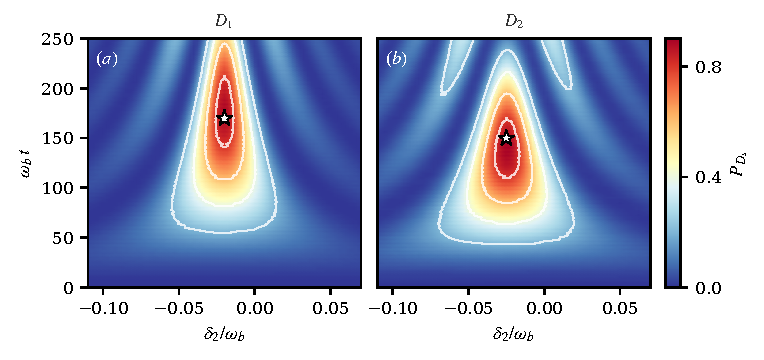
\includegraphics[width=0.86\textwidth]{../figs/figM1_raman_response.pdf}
\caption{Respuesta de las dos escrituras Raman del protocolo temporal;
el óptimo depende de la desintonía de dos fotones y de la duración.}
\label{fig:M1}
\end{figure}
\begin{figure}[htbp]\centering
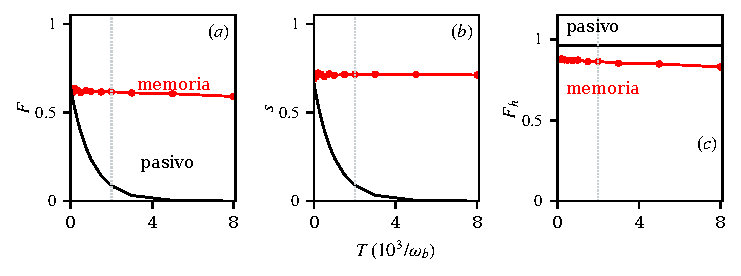
\includegraphics[width=0.94\textwidth]{../figs/figM2_operational_sweep.pdf}
\caption{Resultado operativo F17c del modelo reducido: fidelidad sin
condicionar, probabilidad de recuperación y fidelidad condicionada
frente al tiempo, con $\kappa_{\rm in}=\kappa_{\rm out}=10\kappa$, $\kappa=10^{-3}$, $\gphi=4\times10^{-4}$, $\chi=1$ y pulsos F13 fijos. Puntos: soluciones F17c; la línea los une. La referencia pasiva es analítica con los mismos puertos.}
\label{fig:M2}
\end{figure}
\begin{figure}[htbp]\centering
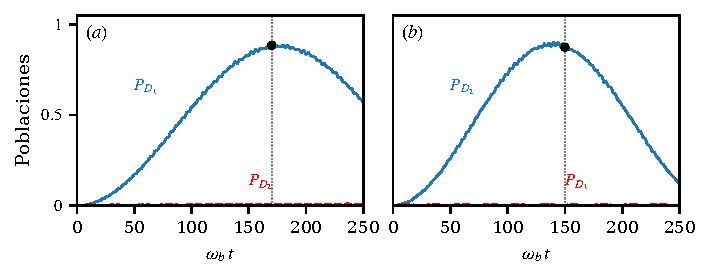
\includegraphics[width=0.86\textwidth]{../figs/figM3_raman_dynamics.pdf}
\caption{Población de la ranura oscura objetivo y diafonía hacia la otra
ranura durante cada pulso Raman. La figura no representa la población
virtual del brillante.}
\label{fig:M3}
\end{figure}
\begin{figure}[htbp]\centering
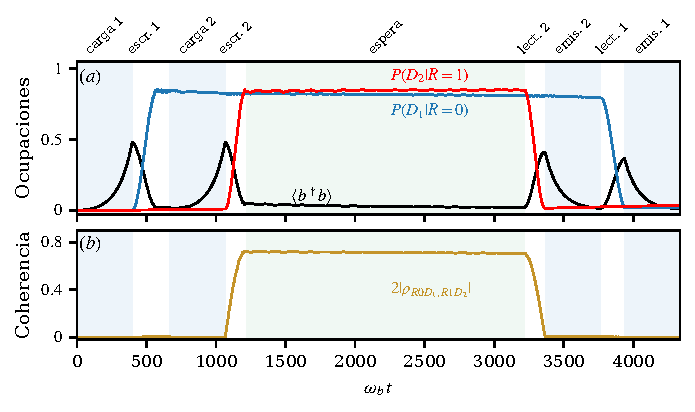
\includegraphics[width=0.94\textwidth]{../figs/figM4_protocol_dynamics.pdf}
\caption{Dinámica por etapas de carga, escritura, espera y lectura para
el protocolo de \emph{time-bins} con puertos reales de F17c.}
\label{fig:M4}
\end{figure}
\begin{figure}[htbp]\centering
\includegraphics[width=0.90\textwidth]{../figs/figM5_dark_storage_decay.pdf}
\caption{Decaimiento de las poblaciones oscuras y de su coherencia.
El ruido común protege la coherencia $D_1$--$D_2$ durante la espera;
el ruido local no.}
\label{fig:M5}
\end{figure}

\bibliographystyle{unsrt}
\bibliography{../REFERENCIAS}
\end{document}
